\newpage
\section{Криптографическая составляющая EAP-PSK}

EAP-PSK реализован с использованием единственного криптографического примитива - блочного шифра из семейства AES-128. На вход AES-128 принимает 16-байтный предустановленный ключ и блок открытого текста размером 16 байт. После работы алгоритм возвращает 16 байт шифртекста. Детальное описание шифра AES-128 можно увидеть в документе ``Specification for the Advanced Encryption Standard (AES)'' 

AES-128 был выбран потому что:
\begin{itemize}
\item его стандарты и реализации находятся в публичном доступе;
\item алгоритм тщательно изучился криптографическим сообществом и считается безопасным.
\end{itemize}

При реализации EAP-PSK могут использоваться и другие блочные шифры, протокол не зависит от AES-128. Единственными параметрами AES-128 от которых зависит EAP-PSK являются длина ключа и размер блока текста (16 байт). Однако, дял простоты реализации было принято решение использовать только один алгоритм шифрования и не допускать обмена данными во время работы протокола с целью выбора алгоритма из множества. В том случае, если AES-128 окажется устаревшим с точки зрения инфомрационной безопасности, EAP-PSK так же устареет и его необходимо будет заменить протоколом EAP-PSK' который будет использовать другой блочный алгоритм шифрования. EAP-PSK' не должен быть обратно совместим с EAP-PSK из-за сообрежиний безопасности. Следовательно EAP-PSK' должен использовать другие значения поля TYPE в EAP-Reqest/Response. Значения поля TYPE в EAP-Reqest/Response описанны в RFC3748. Использование новых значений поля TYPE будет препятствовать появлению появлению уязвимости выбора протокола.

EAP-PSK использует криптографию для:
\begin{itemize}
\item Установка ключей, во время которй вырабатывается AK и KDK;
\item Обмен ключами аутентификации для взаимной аутентификации и выработки сессионного ключа;
\item Для защиты канала обмена данными во время процедуры аутентификации.
\end{itemize}

Каждый пункт рассмотрен подробнее в последующих пунктах.

\subsection{Установка ключей}

EAP-PSK использует два криптографически разделимых 16-байтовых ключа для взаимной аутентификации и генерации сессионных ключей. На самом деле это один из принципов критпографии - использовать разные ключи для разных операций.

Эти ключи можно получить разделив на две части 32-байтовый PSK или использовать 16-байтовый PSK, который будет криптографически расширен до 32-байт и разделен на две части.

Так как распределение долгосрочных идентификационных данных длиной в 32 байта сложнее чем распределение 16-байтовых данных, а так же сессионные ключи всё равно имеют длину в 16 байт, был выбран второй вариант.

Таким образом, PSK используется только для генерации AK и KDK. При этом, оба ключа генерируются только один раз, сразу же после получения PSK. После того как AK и KDK были сгенерированы, PSK следует удалить. Удаление ключа должно гарантировать невозможность его восстановления (руководство по удалению ключей представлено в документе ``National Industrial Security Program Operating Manual'')

Процедура генерации AK и KDK из PSK называется этапом установки ключей:

\begin{itemize}
\item на вход принемается PSK;
\item на выходе AK и KDK.
\end{itemize}

AK и KDK генерируются из PSK с использованием AES-128 в режиме счетчика (CTR). Режим счетчика позволяет расширить входной блок в t раз, где t >= 2. Этот режим был выбран для этапа установки ключей так как этот же режим используется для генерации сессионных ключей (раздел 3.2).

Детали алгоритма генерации AK и KDK представлены на рисунке \ref{img:key_derivation}.

\begin{figure}[h!]
\center{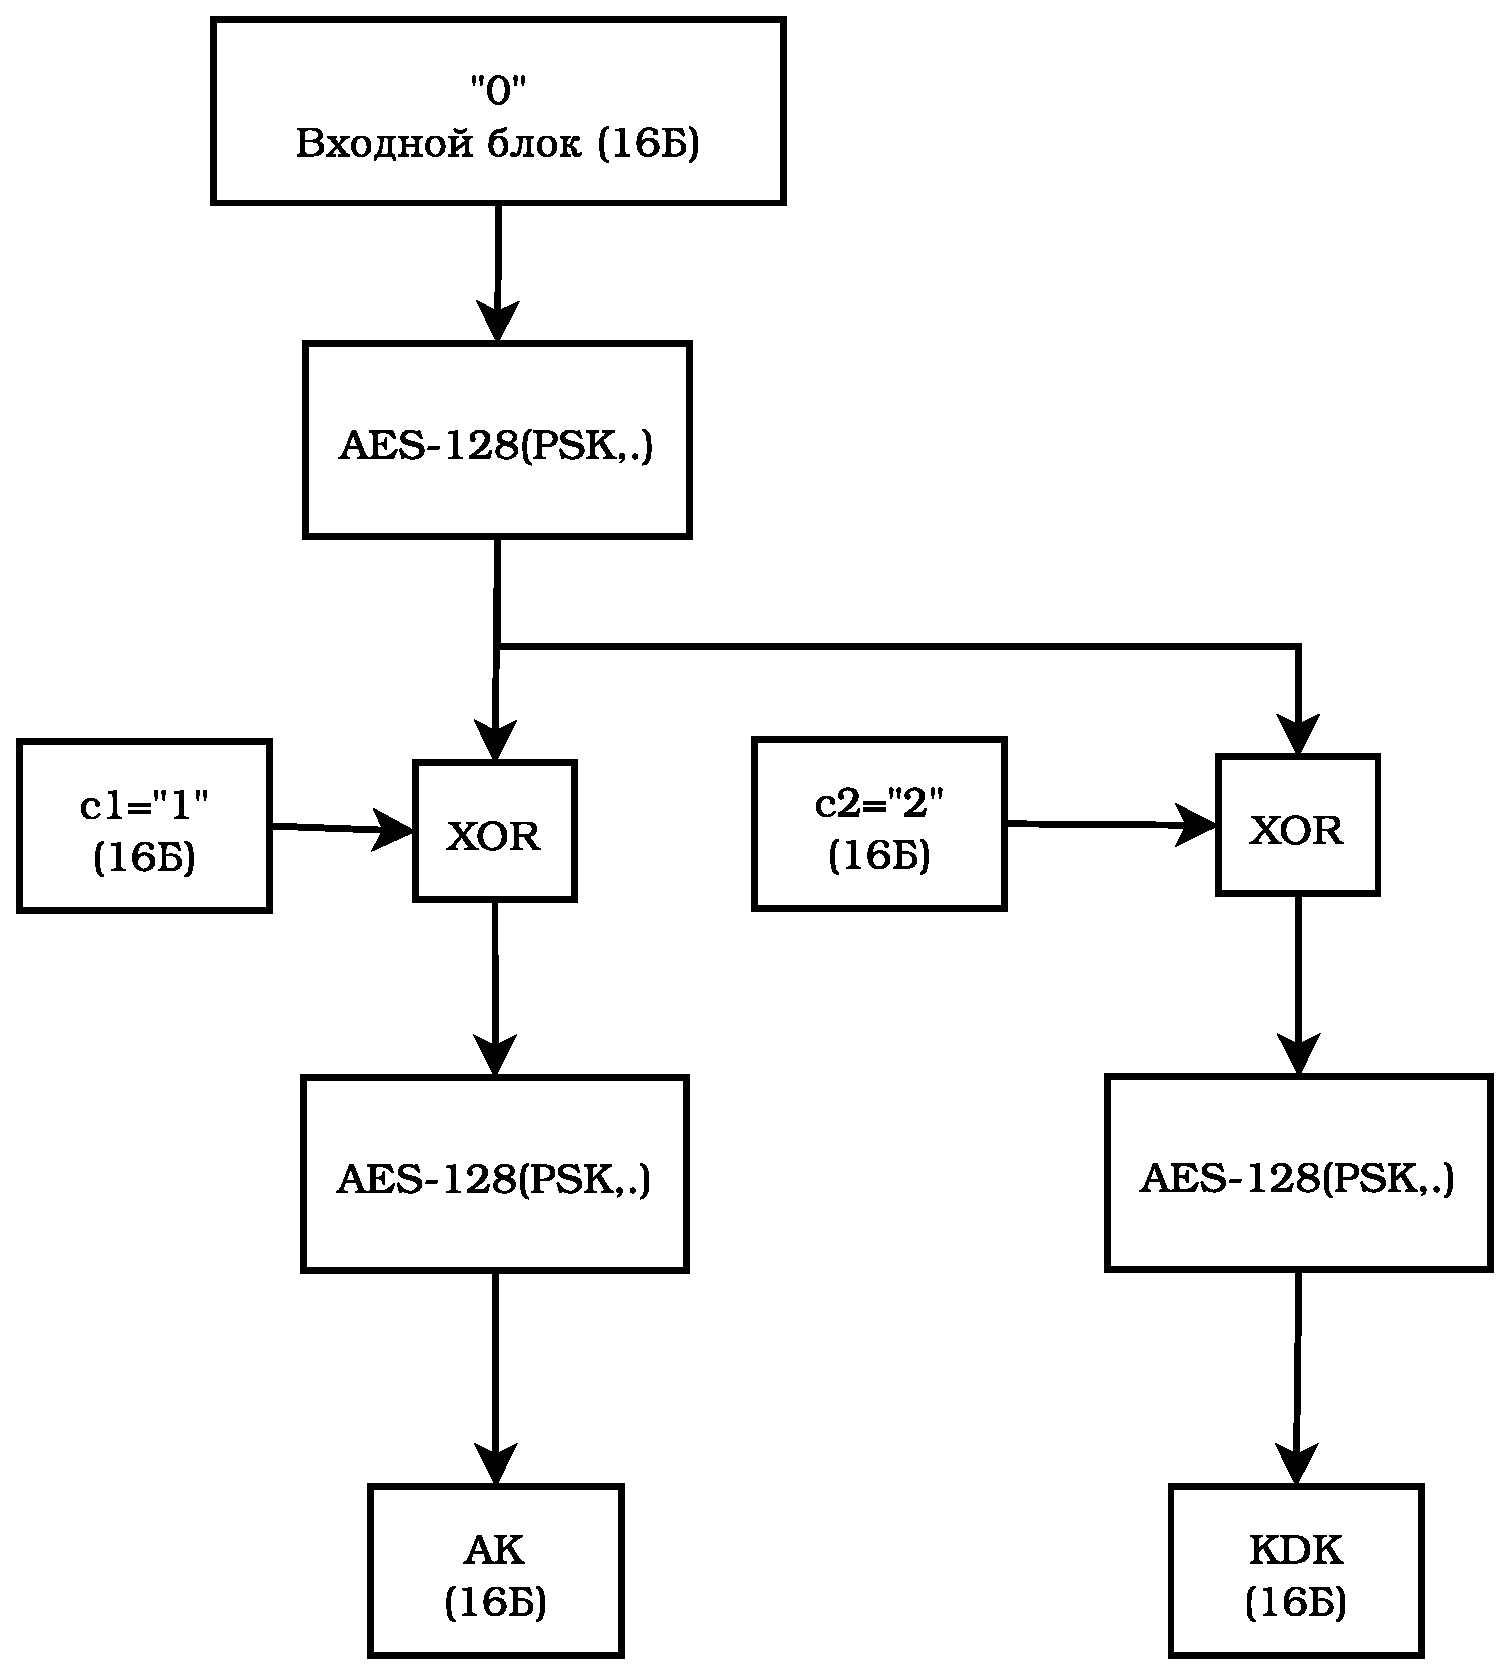
\includegraphics[width=0.9\linewidth]{./pictures/key_derivation}}
\caption{Генерация AK и KDK из PSK}
\label{img:key_derivation}
\end{figure}

Входным блок, для простоты, всегда является ``0''. Данное значение можно расчитывать в завиимости от Пира исервера (например XOR от значений из NAI), но это не дает значительного увеличения безопасности и значительно усложняет схему. Для работы может быть выбрана любая константа, это не влияет на свойства безопасности. Разработчики просто выбрали ``0''.

\subsection{Обмен ключами аутентификации}

В EAP-PSK для аутентификации используется алгоритм, схожий с AKEP2, который описан в документе ``Entity Authentication and Key Distribution'' (EAKD).

AKEP2 состоит из полутора раундов обмена, которые представлены на рисунке \ref{img:akep2}.

\begin{figure}[h!]
\center{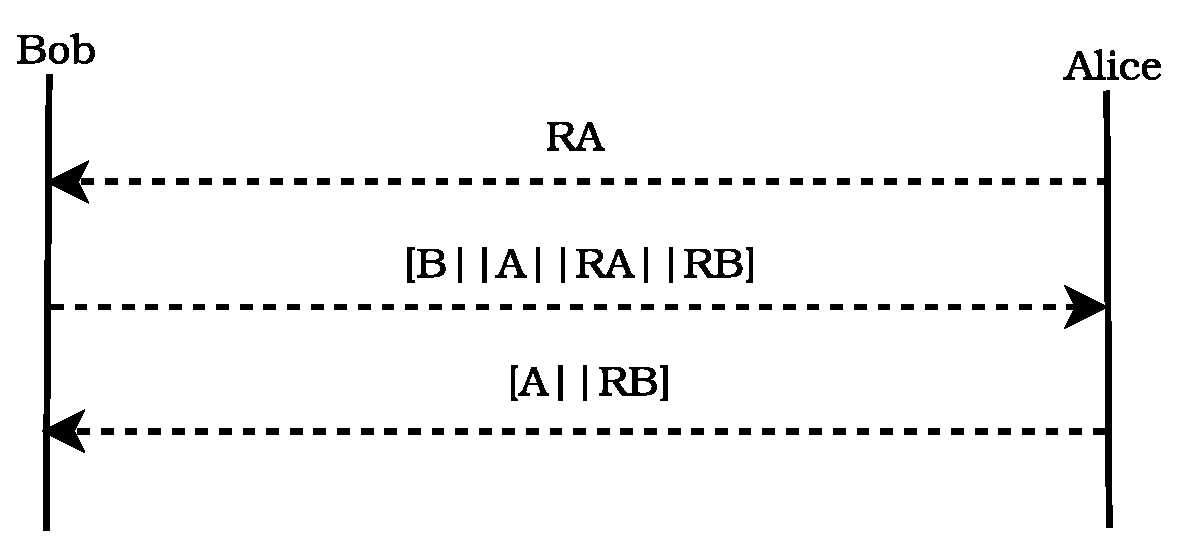
\includegraphics[width=0.9\linewidth]{./pictures/akep2}}
\caption{Описание AKEP2}
\label{img:akep2}
\end{figure}

Стоит отметить, что EAKD фокусируется на теоритической критпографии, а не на протоколах используемых в реальных условиях. Как описано в разделе ``Out-Of-Band-Data'' EAKD, Алиса отправляет A (её идентификатор) Бобу, затем Боб может выбрать соответствующие данные для продолжения обмена. Для EAP-PSK механизм изменен. AKEP2 для EAP-PSK представлен на рисунке \ref{img:eap-akep2}.

\begin{figure}[h!]
\center{\includegraphics[width=0.9\linewidth]{./pictures/eap-akep2}}
\caption{Описание AKEP2 для EAP-PSK}
\label{img:eap-akep2}
\end{figure}
